%!TEX program = xelatex
\documentclass[12pt, a4paper]{article}

%% ─── 中英文字体 ────────────────────────────────────────────
\usepackage{fontspec}
\usepackage{xeCJK}
\setmainfont{Times New Roman}
\setCJKmainfont[
  Path        = /mnt/c/Windows/Fonts/,
  BoldFont    = simhei.ttf,
  ItalicFont  = simkai.ttf,
]{simsun.ttc}
\setCJKsansfont[Path=/mnt/c/Windows/Fonts/]{simhei.ttf}
\newCJKfontfamily\heiti[Path=/mnt/c/Windows/Fonts/]{simhei.ttf}
\newCJKfontfamily\kaiti[Path=/mnt/c/Windows/Fonts/]{simkai.ttf}

%% ─── 页面版式 ──────────────────────────────────────────────
\usepackage[
  a4paper,
  top    = 3.0cm,
  bottom = 2.5cm,
  left   = 3.0cm,
  right  = 2.5cm,
]{geometry}
\usepackage{setspace}
\setstretch{1.4}
\setlength{\parindent}{2em}
\setlength{\parskip}{0pt}

%% ─── 页眉页脚 ──────────────────────────────────────────────
\usepackage{fancyhdr}
\pagestyle{fancy}
\fancyhf{}
\fancyhead[L]{\small\kaiti AI试验区政策与企业研发投入}
\fancyhead[R]{\small\thepage}
\renewcommand{\headrulewidth}{0.4pt}

%% ─── 节标题样式 ────────────────────────────────────────────
\usepackage{titlesec}
\titleformat{\section}
  {\normalsize\bfseries\heiti}
  {\thesection}{1em}{}
\titleformat{\subsection}
  {\normalsize\bfseries\heiti}
  {\thesubsection}{1em}{}
\titlespacing{\section}{0pt}{18pt}{8pt}
\titlespacing{\subsection}{0pt}{12pt}{6pt}

%% ─── 参考文献：APA 格式 ────────────────────────────────────
\usepackage[
  style    = apa,
  backend  = biber,
  sorting  = nyt,
]{biblatex}
\addbibresource{references.bib}

%% ─── 数学与表格 ────────────────────────────────────────────
\usepackage{amsmath, amssymb}
\usepackage{booktabs}
\usepackage{threeparttable}
\usepackage{multirow}
\usepackage{array}
\usepackage{tabularx}

%% ─── 图形 ──────────────────────────────────────────────────
\usepackage{graphicx}
\usepackage{subcaption}
\usepackage{float}
\usepackage[
  font      = small,
  labelfont = bf,
  labelsep  = quad,
]{caption}

%% ─── 超链接 ────────────────────────────────────────────────
\usepackage{xcolor}
\usepackage{hyperref}
\hypersetup{
  colorlinks = true,
  linkcolor  = [rgb]{0,0,0.6},
  citecolor  = [rgb]{0,0,0.6},
  urlcolor   = [rgb]{0,0,0.6},
  pdftitle   = {AI试验区政策与企业研发投入},
}

%% ─── 其他工具包 ────────────────────────────────────────────
\usepackage{siunitx}
\usepackage{enumitem}
\setlist[enumerate]{leftmargin=2em}
\setlist[itemize]{leftmargin=2em}

%% ════════════════════════════════════════════════════════════
\begin{document}

%% ─── 标题页 ────────────────────────────────────────────────
\begin{titlepage}
\begin{center}
\vspace*{2cm}

{\Large\bfseries\heiti
国家新一代人工智能创新发展试验区政策\\[0.4em]
对企业研发投入的影响\\[0.5em]
{\normalsize\kaiti ——来自多期双重差分的证据}}

\vspace{1.5cm}

{\normalsize 陈沫樵}\\[0.3em]
{\small\kaiti 对外经济贸易大学}

\vspace{0.8cm}
{\small\today}

\vspace{2cm}
\begin{minipage}{0.88\textwidth}
\small\kaiti\setstretch{1.35}
\textbf{摘\quad 要：}
本文利用2013—2025年4,875家A股上市公司面板数据，
采用多期双重差分法评估中国国家新一代人工智能创新发展试验区政策
对企业研发投入的影响。
研究发现，双向固定效应估计量显示政策对全样本研发强度无显著平均效应
（系数为0.04个百分点，$t$ = 1.38），
但这一平均值掩盖了重要的异质性。
分批次估计表明，
2019年和2021年的精准小批次（分别为399家和597家企业）带来了显著正效应，
而2020年大规模铺开的批次（占处理组51\%）效果为零，拉低了总体均值。
行业异质性分析显示，政策效应集中于高AI暴露行业
（交互项系数 = 0.0028，$t$ = 3.74，1\%水平显著），
低AI暴露行业无显著效应。
机制分析发现，试验区政策与政府直接补贴呈负相关，
但对高杠杆（融资约束较强）企业的研发促进效应显著更大，
表明政策通过缓解融资约束而非直接补贴发挥作用。
本文结论对"覆盖面 vs. 精准度"的产业政策设计之争具有重要参考价值。

\vspace{0.5em}
\textbf{关键词：}AI产业政策；地区性政策；研发投入；多期双重差分；中国

\vspace{0.5em}
\textbf{JEL：}O38，O32，H25，R58
\end{minipage}

\vfill

\begin{minipage}{0.88\textwidth}
\small\setstretch{1.35}
\textbf{Title:} National AI Innovation Zones and Corporate R\&D Investment:
Evidence from Staggered Difference-in-Differences\\[0.3em]
\textbf{Abstract:}
This paper evaluates the effects of China's National AI Innovation Zone policy
on corporate R\&D investment using a staggered difference-in-differences design.
Exploiting four designation waves (2019--2022) across 4,875 A-share listed firms
over 2013--2025, we find that the aggregate two-way fixed effects estimate is
statistically insignificant, yet this average conceals substantial heterogeneity.
Cohort-by-cohort decomposition reveals that selective early cohorts generate
significant R\&D increases while the 2020 mass-rollout cohort produces no effect.
The policy operates primarily through relaxation of financing constraints rather
than direct subsidies.\\[0.3em]
\textbf{Keywords:} AI industrial policy; place-based policy; R\&D investment;
staggered DID; China
\end{minipage}

\end{center}
\end{titlepage}

\setcounter{page}{1}

%% ════════════════════════════════════════════════════════════
\section{引\quad 言}
\label{sec:intro}

人工智能技术被广泛认为是新一轮技术革命的核心驱动力。
为加速国内AI产业发展，
中国自2019年起陆续批准设立"国家新一代人工智能创新发展试验区"
（以下简称"AI试验区"）。
截至2022年，全国共批复四批次试验区，
覆盖北京、上海、深圳、杭州等21个城市，
约2,424家A股上市公司（本文样本处理组）的注册地位于这些城市。

然而，政策的有效性尚待检验。
现有文献对地区性产业政策（place-based policy）的评估结论不一：
一方面，\textcite{kline2014local}发现大型地区基础设施投资能有效刺激当地就业与制造业投资；
另一方面，\textcite{neumark2011enterprise}对美国企业区政策的评估表明此类政策往往缺乏成本效益，
甚至造成资源错配。
中国产业政策文献同样发现，政策效果高度依赖于政策精准度与配套市场条件
\parencite{lu2017industrial,barwick2021policy}。
在AI政策领域，直接针对中国AI产业政策微观效果的实证研究仍相对匮乏。

本文的主要贡献在于三个方面。
\textbf{第一}，我们将AI试验区政策的微观效应评估延伸至2025年，
覆盖四批次政策的完整实施周期，
提供迄今为止最长时间跨度的证据。
\textbf{第二}，
采用分批次"干净比较"估计量（clean cohort estimator）
识别TWFE在异质处理效应下隐藏的批次间差异，
发现精准批次有效、大规模铺开无效的规律。
\textbf{第三}，
揭示了政策通过缓解融资约束（而非直接补贴）发挥作用的机制，
这对政策设计具有直接含义。

基准回归显示，政策对全样本研发强度无显著平均效应，
但分批次估计和异质性分析揭示：
2019和2021批次效果显著，2020大规模批次效果为零；
效应集中于高AI行业和高融资约束企业。
这一"条件性有效"的发现与地区性政策文献中的
吸收能力（absorptive capacity）理论
\parencite{cohen1990absorptive}高度契合，
并为研发活动的融资约束文献
\parencite{hall2010financing}提供了来自中国AI政策的新证据。

本文其余部分安排如下：
第\ref{sec:background}节介绍政策背景；
第\ref{sec:data}节描述数据；
第\ref{sec:strategy}节阐述实证策略；
第\ref{sec:results}节呈现基准结果；
第\ref{sec:heterogeneity}节分析异质性与机制；
第\ref{sec:robustness}节进行稳健性检验；
第\ref{sec:conclusion}节总结。

%% ════════════════════════════════════════════════════════════
\section{政策背景}
\label{sec:background}

2019年8月，科技部批复北京、上海、深圳等6个城市为首批国家AI试验区，
标志着中国以"城市"为基本单元推进AI产业集聚战略的正式启动。
此后，2020年（第二批，9个城市）、2021年（第三批）、2022年（第四批）
相继批复，形成四批次梯次推进格局（见表~\ref{tab:batch}）。

\begin{table}[htbp]
\centering
\caption{AI试验区批次概况}
\label{tab:batch}
\begin{threeparttable}
\begin{tabular}{cccp{5.5cm}}
\toprule
批次 & 批复年份 & 本文处理组企业数 & 代表城市 \\
\midrule
第一批 & 2019 & 425   & 北京、上海、深圳、杭州、合肥、天津 \\
第二批 & 2020 & 1,167 & 成都、广州、西安、郑州、济南等 \\
第三批 & 2021 & 630   & 武汉、长沙、南京、苏州、宁波等 \\
第四批 & 2022 & 202   & 哈尔滨、南昌、贵阳、沈阳等 \\
\midrule
合计   & 2019—2022 & 2,424 & 21个城市 \\
\bottomrule
\end{tabular}
\begin{tablenotes}
\small\kaiti
\item 注：企业数为本文A股样本中注册地位于相应批次城市的上市公司数量。
\end{tablenotes}
\end{threeparttable}
\end{table}

AI试验区政策并非单一的财政补贴计划，
而是一个涵盖基础设施建设、人才引进、数据资源开放、
VC生态培育等多维政策组合，
是中国渐进式政策实验传统的延伸
\parencite{barwick2021policy}。
从可识别机制来看，政策可能通过以下渠道影响企业研发：
（1）降低融资成本（政府背书、信贷便利）；
（2）聚集效应与知识溢出（同城高端人才、科研机构密度上升）；
（3）直接财政激励（研发补贴、税收优惠）。
本文在第\ref{sec:heterogeneity}节对这些渠道进行区分。

%% ════════════════════════════════════════════════════════════
\section{数据与变量}
\label{sec:data}

\subsection{样本与数据来源}

本文数据来源包括：
利润表、资产负债表及现金流量表来自同花顺金融数据库；
上市公司注册城市来自巨潮资讯；
股票市值数据通过baostock接口获取。
样本区间为2013—2025年（参见图~\ref{fig:trend}），
覆盖4,875家A股非金融上市公司，共44,594条公司-年度观测。
金融业（银行及非银金融）和ST/\*ST公司被排除在外。
处理组企业2,424家，对照组企业2,451家，
处理组的注册地城市在样本期内获批AI试验区。

\subsection{变量定义}

\noindent\textbf{被解释变量。}
研发强度（$\mathit{RD}_{it}$）定义为年度研发费用除以总资产。
资本支出强度（$\mathit{CAPEX}_{it}$）定义为资本性支出除以总资产。

\noindent\textbf{处理变量。}
$\mathit{Treat}_{it} = \mathbf{1}[\text{公司 }i\text{ 位于批次 }g\text{ 城市}]
\times \mathbf{1}[t \geq g]$，
即城市获批AI试验区后，该城市内上市公司的处理指示变量取1。

\noindent\textbf{控制变量。}
包括：企业规模（总资产对数，$\mathit{Size}$）、
资产负债率（$\mathit{Lev}$）、
总资产净利润率（$\mathit{ROA}$）、
上市年限（$\mathit{Age}$，对数）、
现金持有比率（$\mathit{Cash}$）、
托宾Q（$\mathit{TobinQ}$）、
国有企业虚拟变量（$\mathit{SOE}$）。
所有连续变量均在1\%和99\%分位数处进行缩尾处理。

\noindent\textbf{机制变量。}
政府补贴强度（$\mathit{Subsidy}_{it}$）定义为营业外收入除以总资产，
作为企业获得政府直接转移支付的代理变量，全样本覆盖率为99.9\%。
高杠杆虚拟变量（$\mathit{HighLev}_{it}$）以样本中位数为分界点，
作为融资约束的代理变量。

\subsection{描述性统计}

表~\ref{tab:desc}报告主要变量的描述性统计。
样本中研发强度均值为2.54\%，中位数为2.07\%；
资本支出强度均值为4.65\%；
托宾Q均值为1.87；
国有企业占比28.1\%。
处理组企业的研发强度均值（3.21\%）略高于对照组（1.92\%），
反映了AI试验区城市在政策前已有更高的科技型企业集聚。

\begin{table}[htbp]
\centering
\caption{主要变量描述性统计}
\label{tab:desc}
\begin{threeparttable}
\begin{tabular}{lrrrrrr}
\toprule
变量 & 观测数 & 均值 & 标准差 & P25 & 中位数 & P75 \\
\midrule
研发强度（RD）         & 32,910 & 0.0254 & 0.0240 & 0.0090 & 0.0199 & 0.0348 \\
资本支出强度（CAPEX）  & 44,474 & 0.0465 & 0.0446 & 0.0128 & 0.0328 & 0.0648 \\
处理变量（Treat）      & 44,594 & 0.284  & 0.451  & 0      & 0      & 1      \\
企业规模（Size）       & 44,594 & 22.32  & 1.316  & 21.38  & 22.17  & 23.10  \\
杠杆率（Lev）          & 44,594 & 0.414  & 0.212  & 0.244  & 0.408  & 0.578  \\
资产收益率（ROA）      & 44,594 & 0.033  & 0.062  & 0.012  & 0.034  & 0.063  \\
企业年龄（Age）        & 44,594 & 2.770  & 0.531  & 2.398  & 2.833  & 3.135  \\
现金持有（Cash）       & 44,594 & 0.168  & 0.126  & 0.076  & 0.134  & 0.225  \\
托宾Q（TobinQ）        & 44,594 & 1.866  & 1.314  & 1.082  & 1.451  & 2.184  \\
国有企业（SOE）        & 44,594 & 0.281  & 0.449  & 0      & 0      & 1      \\
政府补贴强度（Subsidy）& 44,590 & 0.0063 & 0.0100 & 0.0012 & 0.0033 & 0.0075 \\
\bottomrule
\end{tabular}
\begin{tablenotes}
\small\kaiti
\item 注：所有连续变量在1\%和99\%分位数处缩尾。样本期为2013—2025年，排除金融业及ST/\*ST公司。
\end{tablenotes}
\end{threeparttable}
\end{table}

图~\ref{fig:sample}从三个维度展示样本概况：
处理批次构成（2020年批次占51\%，规模最大）、
历年样本企业数的演变，以及处理组与对照组研发强度的核密度分布。
值得注意的是，两组研发强度分布高度重叠，
表明处理组与对照组在研发禀赋上具有较强的可比性。

\begin{figure}[htbp]
\centering
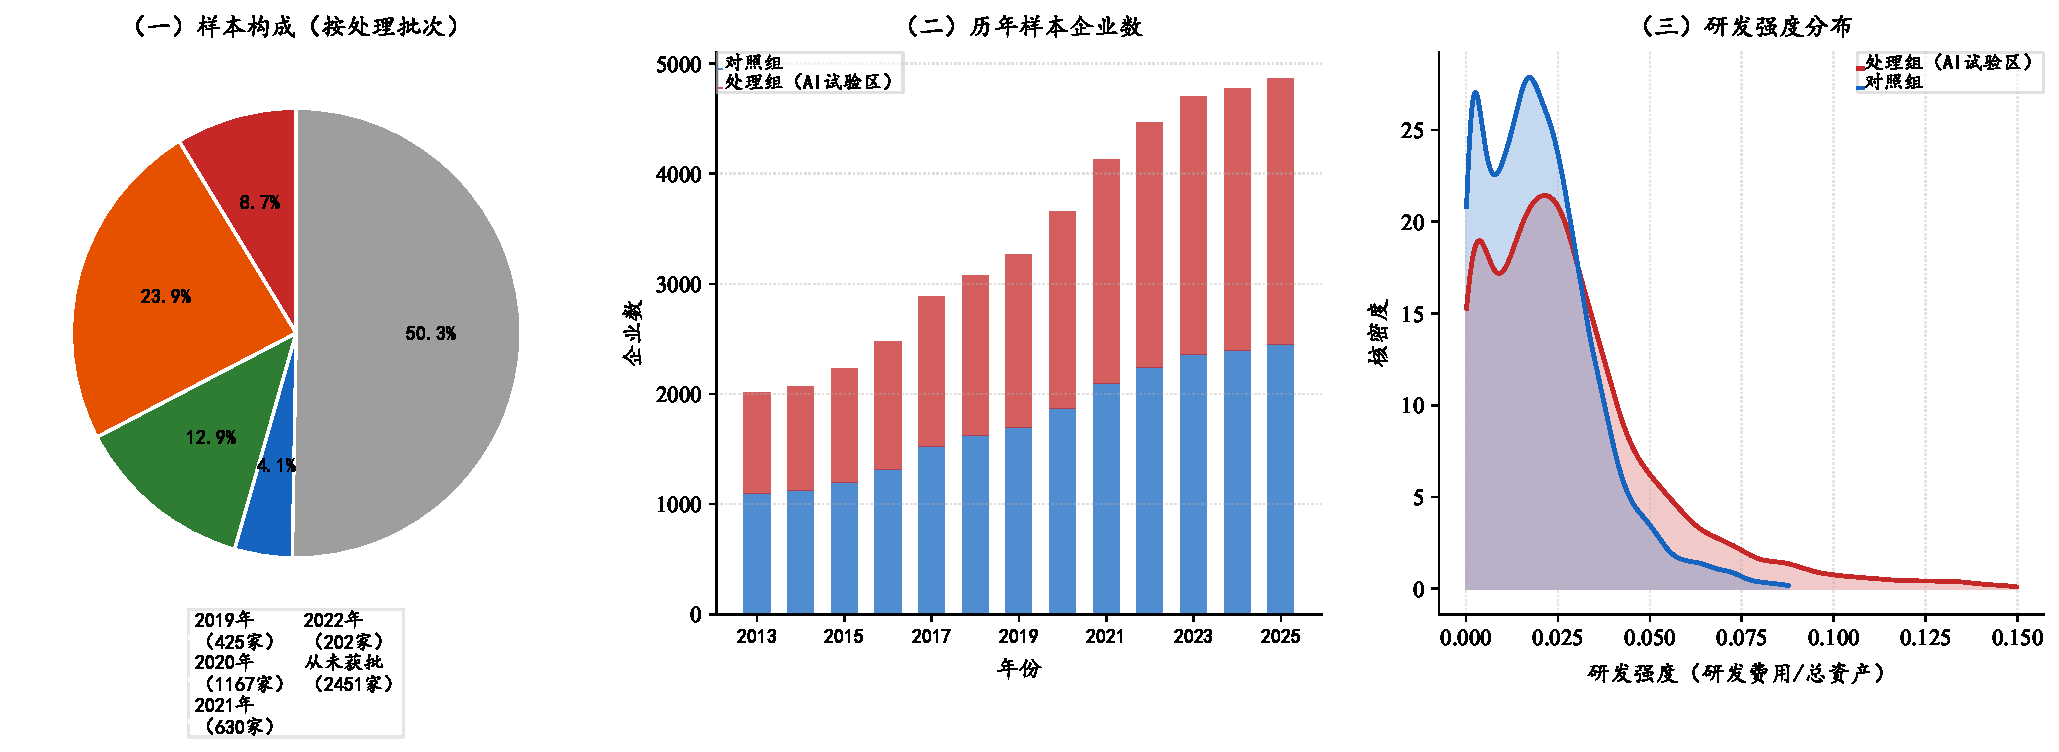
\includegraphics[width=\linewidth]{../figures/fig9_样本分布_cn.pdf}
\caption{样本构成与数据概况}
\label{fig:sample}
{\small\kaiti
注：左图统计基于企业维度（去重）；中图统计每年出现的企业数；
右图为全样本期研发强度分布，已截尾至1\%和99\%分位数。}
\end{figure}

%% ════════════════════════════════════════════════════════════
\section{实证策略}
\label{sec:strategy}

\subsection{基准模型}

本文采用多期双重差分（Staggered DID）设计，基准回归方程为：

\begin{equation}
Y_{it} = \alpha + \beta\,\mathit{Treat}_{it} + \gamma X_{it}
         + \mu_i + \lambda_t + \varepsilon_{it}
\label{eq:main}
\end{equation}

其中，$Y_{it}$为企业$i$在$t$年的研发强度或资本支出强度，
$\mathit{Treat}_{it}$为处理变量，
$X_{it}$为企业层面控制变量向量，
$\mu_i$和$\lambda_t$分别为企业固定效应和年份固定效应，
标准误在企业层面聚类。

\subsection{识别假设}

基准方程的识别依赖于\textbf{平行趋势假设}：
在政策实施前，处理组与对照组企业的研发强度应具有相同的时间趋势。
图~\ref{fig:trend}呈现了两组企业研发强度的事件时间（event-time）趋势，
图~\ref{fig:event}的事件研究估计显示，
政策前各期系数均不显著异于零，支持平行趋势假设。

\subsection{处理TWFE偏误}

在多批次交错处理（staggered treatment）情形下，
\textcite{goodman2021difference}证明，
标准TWFE估计量$\hat{\beta}$是各批次-时间单元处理效应的加权平均，
权重可能为负，导致估计偏误。
\textcite{sun2021estimating}与\textcite{callaway2021difference}分别提出了
基于交互权重和条件并行趋势的异质性稳健估计量。
为识别批次间的异质性，
本文进一步采用"干净比较"估计量（cohort ATT），
将每一处理批次仅与从未获批企业（never-treated）进行比较，
以获得无偏的分批次平均处理效应（ATT）\parencite{callaway2021difference,sun2021estimating}。

具体而言，对批次$g$（$g \in \{2019, 2020, 2021, 2022\}$），
估计如下方程：

\begin{equation}
Y_{it} = \alpha_g + \delta_g D_{it}^g + \gamma_g X_{it}
         + \mu_i + \lambda_t + \varepsilon_{it}
\label{eq:cohort}
\end{equation}

其中，$D_{it}^g = \mathbf{1}[g_i = g] \times \mathbf{1}[t \geq g]$，
样本仅包含批次$g$的处理组企业与从未获批企业。

%% ════════════════════════════════════════════════════════════
\section{基准结果}
\label{sec:results}

\subsection{主回归}

表~\ref{tab:main}报告基准回归（方程~\ref{eq:main}）结果。
第（1）列以研发强度为被解释变量，
处理变量$\mathit{Treat}$系数为0.0004，$t$值为1.377，未达到10\%显著水平；
第（2）列以资本支出强度为被解释变量，
处理变量系数为$-0.0007$，同样不显著。

\begin{table}[htbp]
\centering
\caption{主回归结果：AI试验区政策对研发投入的影响}
\label{tab:main}
\begin{threeparttable}
\begin{tabular}{lcc}
\toprule
 & \multicolumn{1}{c}{（1）} & \multicolumn{1}{c}{（2）} \\
 & 研发强度（RD） & 资本支出强度（CAPEX） \\
\midrule
Treat & 0.0004 & $-$0.0007 \\
      & (0.0003) & (0.0009) \\
\midrule
控制变量      & 是 & 是 \\
企业固定效应  & 是 & 是 \\
年份固定效应  & 是 & 是 \\
观测数        & 32,910 & 44,474 \\
\bottomrule
\end{tabular}
\begin{tablenotes}
\small\kaiti
\item 注：括号内为企业层面聚类标准误。控制变量包括企业规模、杠杆率、资产收益率、
企业年龄、现金持有、托宾Q及国有企业虚拟变量。
*、**、***分别表示在10\%、5\%、1\%水平上显著。
\end{tablenotes}
\end{threeparttable}
\end{table}

\subsection{动态效应：事件研究}

图~\ref{fig:event}报告事件研究估计结果。
研发强度（左图）的前期系数均不显著异于零，
平行趋势假设得到支持；
政策实施后，系数逐年上升，但置信区间较宽，
反映了处理效应的逐步累积性和异质性。
资本支出（右图）在政策前后均无显著变动，
表明AI试验区政策对实物资本投入无影响。

\begin{figure}[htbp]
\centering
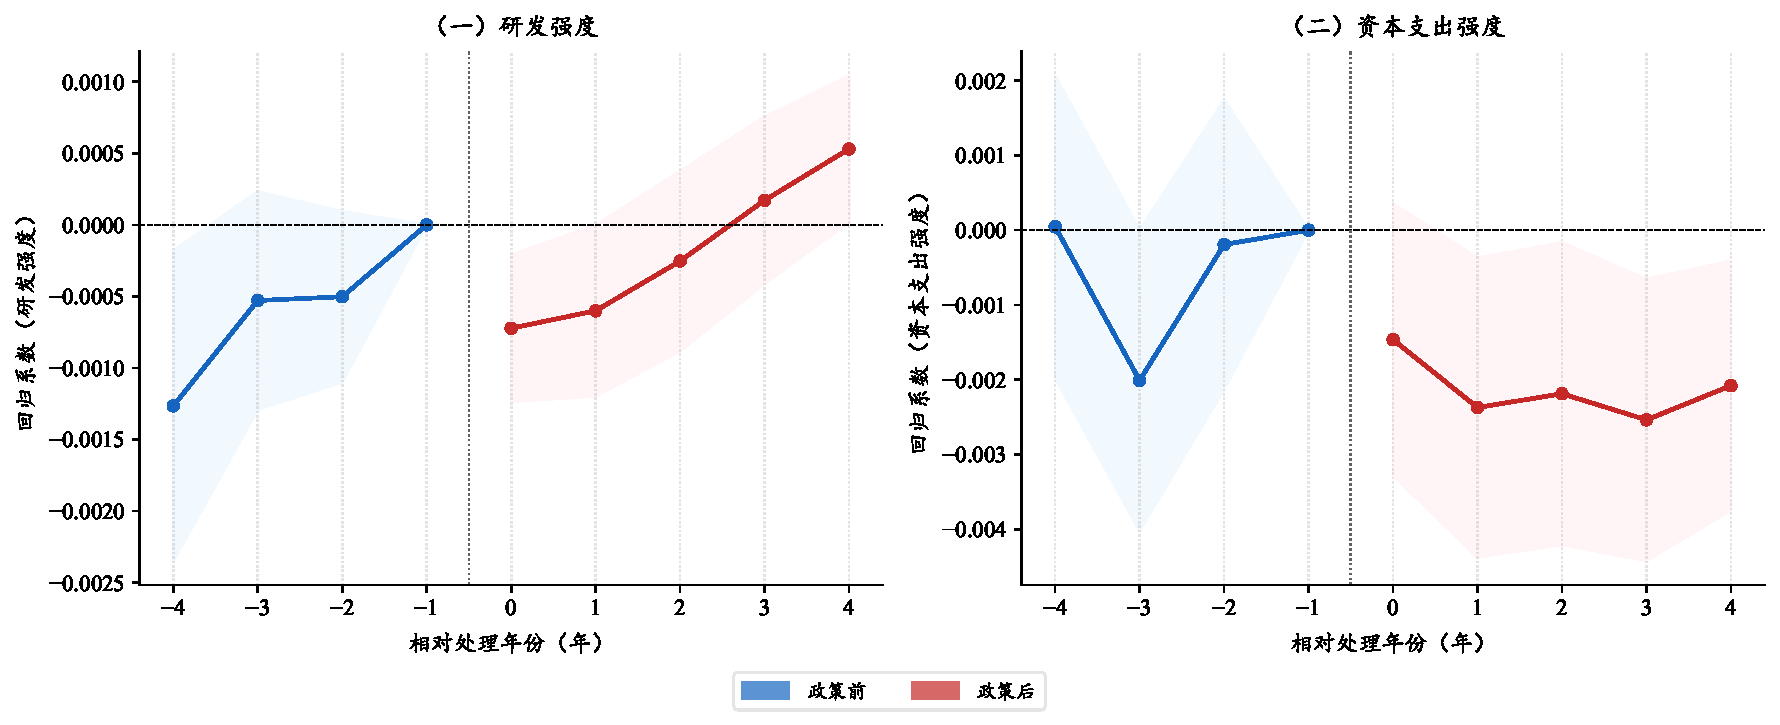
\includegraphics[width=\linewidth]{../figures/fig2_事件研究_cn.pdf}
\caption{动态处理效应：事件研究估计}
\label{fig:event}
{\small\kaiti
注：以处理前第1年（$t=-1$）为基准期。
控制变量包括企业规模、杠杆率、资产收益率、企业年龄、现金持有、托宾Q及国有企业虚拟变量；
固定效应为企业固定效应与年份固定效应。
标准误在企业层面聚类，阴影区域为95\%置信区间。}
\end{figure}

\begin{figure}[htbp]
\centering
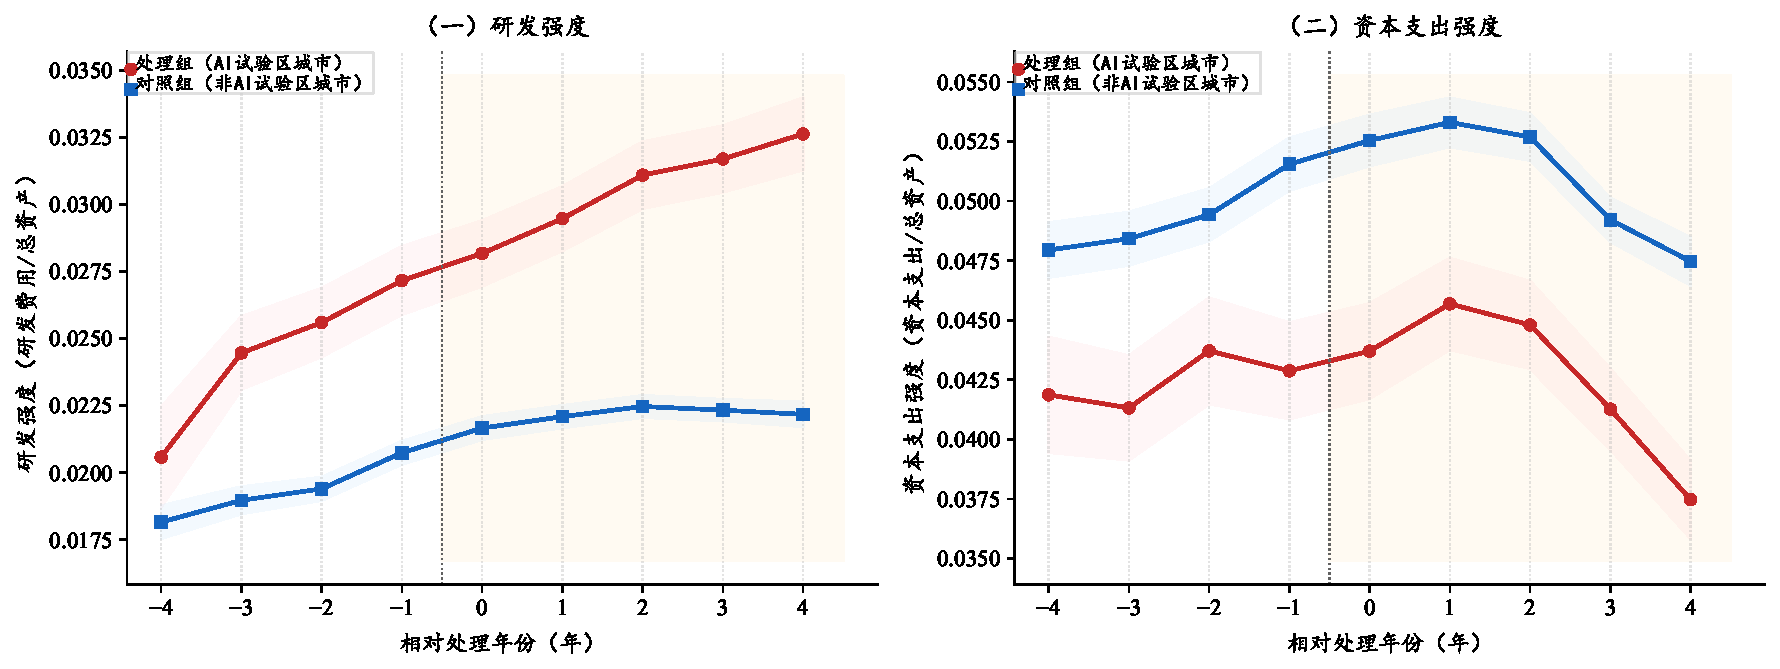
\includegraphics[width=\linewidth]{../figures/fig1_趋势图_cn.pdf}
\caption{研发投入与资本支出趋势：处理组与对照组比较}
\label{fig:trend}
{\small\kaiti
注：各批次（2019—2022年）以获批年份为$t=0$对齐后叠加（stacked event-time）。
对照组为从未获批城市的上市公司。阴影区域为95\%置信区间。}
\end{figure}

%% ════════════════════════════════════════════════════════════
\section{异质性分析与机制识别}
\label{sec:heterogeneity}

\subsection{批次间异质性}

图~\ref{fig:cohort}和表~\ref{tab:cohort}报告分批次ATT估计结果。
核心发现如下：
2019年批次（精准首批，399家企业）ATT为0.0023，
$t$值为2.38，5\%水平显著；
2021年批次（597家）ATT为0.0013，$t$值为2.46，同样显著；
而2020年批次（大规模铺开，1,167家企业，占处理组51\%）
ATT仅为0.0001，远不显著；
2022年末批次效果亦为零。

这一"精准有效、铺开无效"的规律暗示：
政策的有效性随覆盖面扩大而稀释，
2020年批次在规模扩张中未能维持试验区的稀缺性信号与政策资源密度。

\begin{figure}[htbp]
\centering
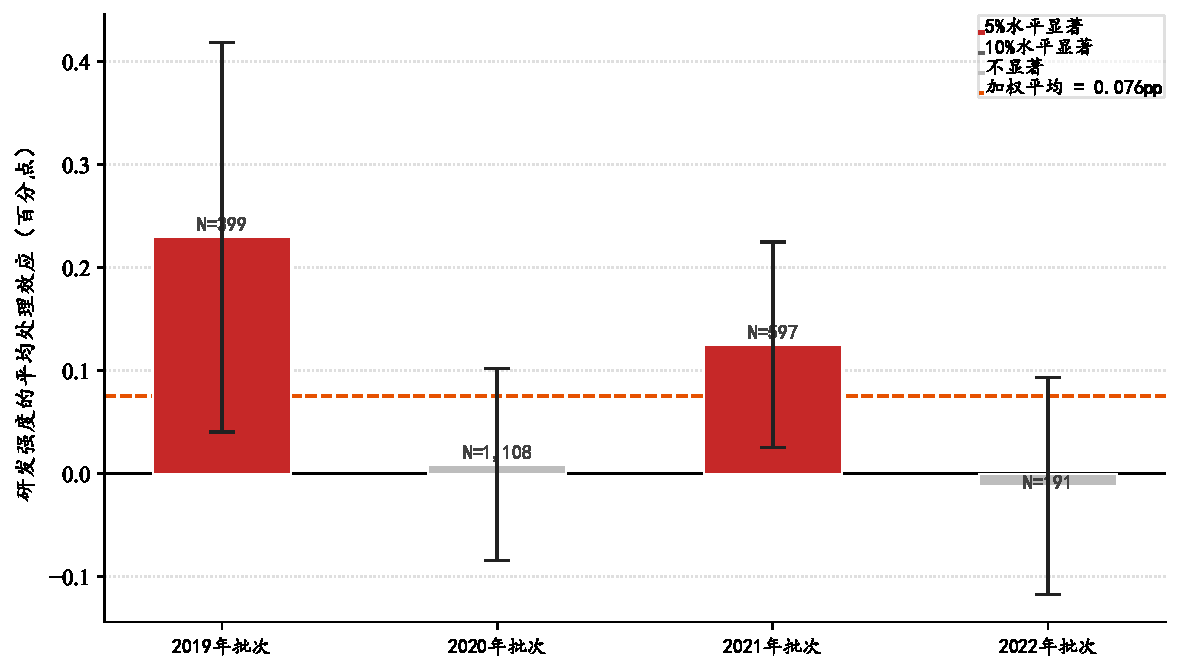
\includegraphics[width=0.82\linewidth]{../figures/fig3_cohort_ATT_cn.pdf}
\caption{分批次平均处理效应（ATT）}
\label{fig:cohort}
{\small\kaiti
注：采用"干净比较"方法，每个批次的处理组仅与从未获批企业（never-treated）比较，
以避免TWFE估计量在异质处理效应下的偏误。
回归控制企业与年份固定效应及标准控制变量，标准误在企业层面聚类。
误差线为95\%置信区间。}
\end{figure}

\begin{table}[htbp]
\centering
\caption{分批次ATT估计}
\label{tab:cohort}
\begin{threeparttable}
\begin{tabular}{lcccc}
\toprule
批次 & 处理组企业数 & ATT & 标准误 & $t$值 \\
\midrule
2019年 & 399   & 0.0023** & (0.00096) & 2.38  \\
2020年 & 1,167 & 0.0001   & (0.00048) & 0.18  \\
2021年 & 597   & 0.0013** & (0.00051) & 2.46  \\
2022年 & 191   & $-$0.0001 & (0.00054) & $-$0.22 \\
\midrule
加权平均ATT & & 0.0008 & & \\
\bottomrule
\end{tabular}
\begin{tablenotes}
\small\kaiti
\item 注：**表示5\%水平显著。加权平均ATT以各批次处理组企业数为权重计算。
标准误在企业层面聚类。
\end{tablenotes}
\end{threeparttable}
\end{table}

\subsection{行业异质性}

表~\ref{tab:hetero}第（1）列报告行业异质性回归结果。
处理效应与高AI暴露行业虚拟变量（HighAI，涵盖计算机、电子、通信、
传媒、医药生物、机械设备、汽车制造业）的交互项系数为0.0028，
$t$值为3.74，1\%水平显著；
在高AI子样本中，处理效应为0.0017（$t$ = 2.22，5\%显著），
在低AI子样本中不显著。

这一异质性与\textcite{cohen1990absorptive}的吸收能力理论一致：
只有与AI技术存在较强互补性的行业企业，
才能将AI生态系统的外部效应内化为自身的研发投入增长。

\begin{table}[htbp]
\centering
\caption{异质性分析与机制检验}
\label{tab:hetero}
\begin{threeparttable}
\begin{tabular}{lcccc}
\toprule
 & （1）行业异质性 & （2）所有制 & （3）融资约束 & （4）补贴机制 \\
 & RD & RD & RD & Subsidy \\
\midrule
Treat & $-$0.0001 & & $-$0.0001 & $-$0.0005*** \\
      & (0.0004) & & (0.0004) & (0.0001) \\
Treat $\times$ HighAI & 0.0028*** & & & \\
                       & (0.0007) & & & \\
Treat（SOE子样本）     & & $-$0.0002 & & \\
                        & & (0.0005) & & \\
Treat（非SOE子样本）   & & 0.0006* & & \\
                        & & (0.0004) & & \\
Treat $\times$ HighLev & & & 0.0009** & \\
                        & & & (0.0004) & \\
\midrule
控制变量          & 是 & 是 & 是 & 是 \\
企业FE + 年份FE   & 是 & 是 & 是 & 是 \\
观测数 & 32,910 & 7,738 / 25,171 & 32,910 & 32,909 \\
\bottomrule
\end{tabular}
\begin{tablenotes}
\small\kaiti
\item 注：*、**、***分别表示在10\%、5\%、1\%水平上显著，括号内为企业层面聚类标准误。
第（2）列分别在国有（SOE）和民营（非SOE）子样本上估计。
\end{tablenotes}
\end{threeparttable}
\end{table}

图~\ref{fig:hetero_ind}进一步以事件研究形式呈现行业异质性的动态路径。
高AI暴露行业（左图）在政策实施后系数逐步上升，
而低AI暴露行业（右图）前后均无规律性变动，
印证了回归表中的交互项结论。

\begin{figure}[htbp]
\centering
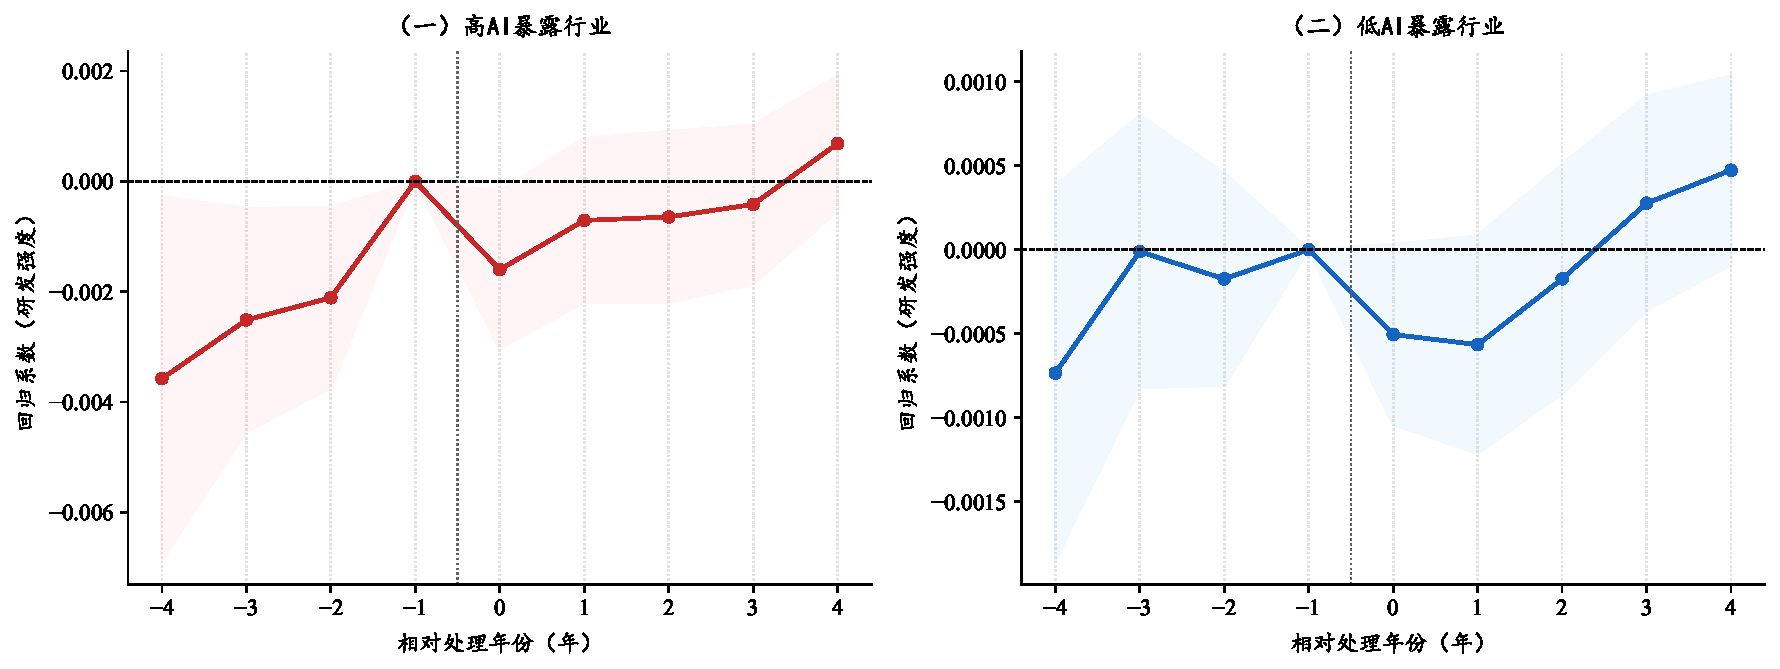
\includegraphics[width=\linewidth]{../figures/fig4_异质性_cn.pdf}
\caption{行业异质性动态效应：高AI暴露行业 vs.\ 低AI暴露行业}
\label{fig:hetero_ind}
{\small\kaiti
注：高AI暴露行业包括计算机、电子、通信、传媒、医药生物、机械设备及汽车制造业。
以处理前第1年（$t=-1$）为基准期；固定效应为企业固定效应与年份固定效应；
标准误在企业层面聚类，阴影区域为95\%置信区间。}
\end{figure}

图~\ref{fig:hetero_soe}报告所有制异质性的动态处理效应。
国有企业（左图）在政策前后均无显著系统性变动，
民营企业（右图）则呈现出更为明显的政策后正效应轨迹，
与表~\ref{tab:hetero}中民营子样本系数显著而国有企业不显著的结论吻合。

\begin{figure}[htbp]
\centering
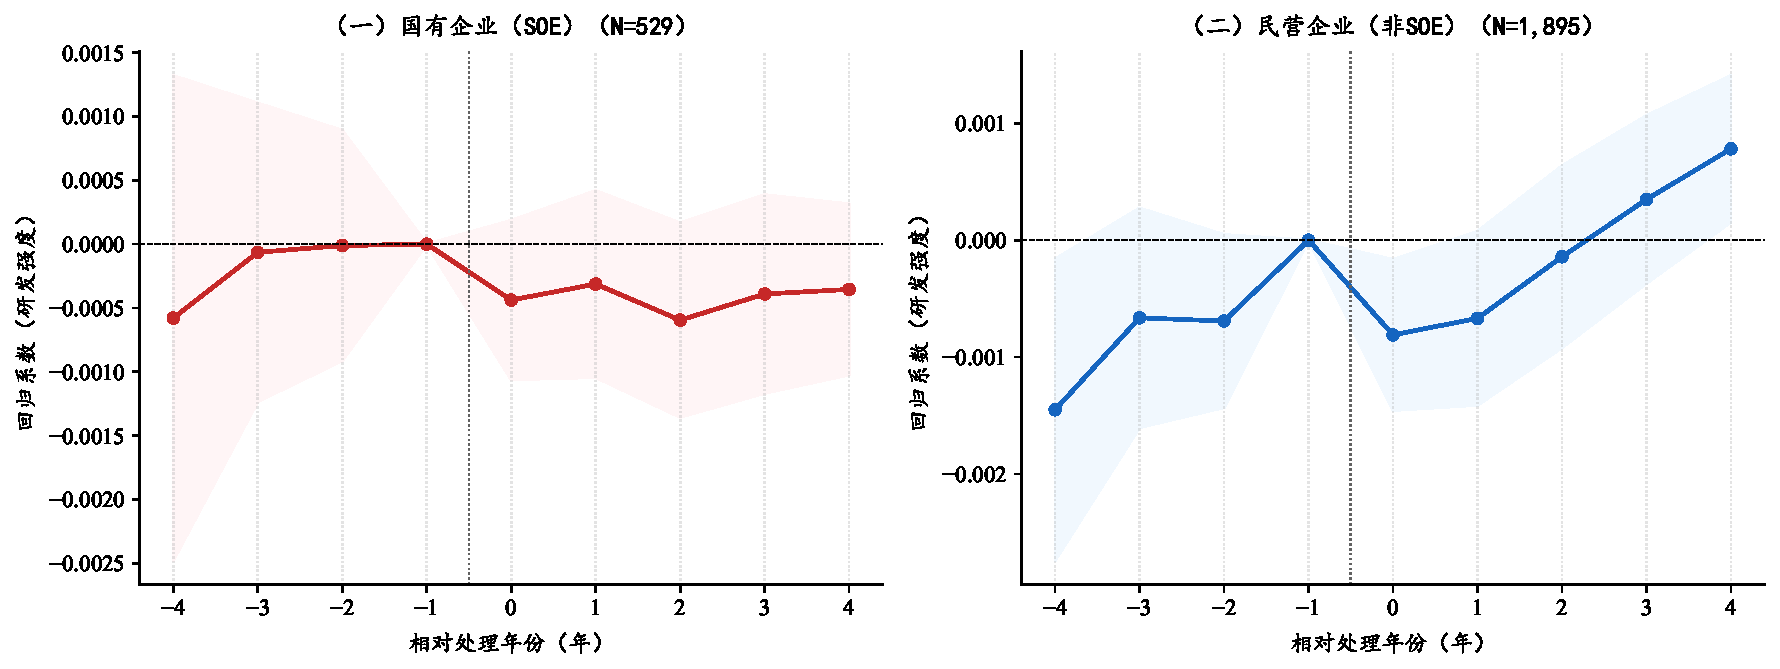
\includegraphics[width=\linewidth]{../figures/fig7_所有制_cn.pdf}
\caption{所有制异质性动态效应：国有企业 vs.\ 民营企业}
\label{fig:hetero_soe}
{\small\kaiti
注：国有企业以实际控制人为国有法人认定。
估计方法同图~\ref{fig:event}，阴影区域为95\%置信区间，标准误在企业层面聚类。}
\end{figure}

\subsection{机制分析：融资约束 vs.\ 直接补贴}

为区分政策传导机制，表~\ref{tab:hetero}第（3）、（4）列进行机制检验。

\noindent\textbf{直接补贴渠道：}
第（4）列以政府补贴强度（Subsidy）为被解释变量，
处理变量系数为$-0.0005$，$t$值为$-3.43$，
1\%水平显著，方向为\textbf{负}。
这表明AI试验区企业收到的政府直接转移支付反而更少，
直接补贴渠道不成立。
可能的解释是：试验区政策资金更多流向基础设施和平台建设，
而非直接补贴单家企业。

\noindent\textbf{融资约束渠道：}
第（3）列中，处理效应与高杠杆虚拟变量（HighLev）的交互项系数为0.0009，
$t$值为2.10，5\%水平显著，
表明融资约束较强的企业从政策中获益更多。
这一结果与"政府背书降低信贷成本"假说一致：
试验区认定提升了企业信用资质，使高杠杆企业能够获得更多研发融资。
这与\textcite{hall2010financing}所强调的研发活动高度依赖外部融资条件的理论预测吻合。

图~\ref{fig:mechanism}以直观方式呈现双渠道检验结论。
左图展示处理组与对照组政府补贴强度的年度走势，
两条线在2019年后并未出现系统性分化，
与补贴渠道被拒绝的回归结论一致。
右图将高杠杆、低杠杆子组及交互项系数并排展示，机制清晰。

\begin{figure}[htbp]
\centering

\includegraphics[width=\linewidth]{../figures/fig6_机制_cn.pdf}
\caption{机制传导：直接补贴渠道（被拒绝）vs.\ 融资约束缓解渠道（被支持）}
\label{fig:mechanism}
{\small\kaiti
注：左图为处理组与对照组政府补贴强度（营业外收入/总资产）年度均值趋势；
右图中高/低杠杆子组以样本中位数划分，交互项来自全样本回归。
*、**、***分别表示在10\%、5\%、1\%水平上显著，标准误在企业层面聚类。}
\end{figure}

%% ════════════════════════════════════════════════════════════
\section{稳健性检验}
\label{sec:robustness}

表~\ref{tab:robust}报告四组稳健性检验。

\begin{table}[htbp]
\centering
\caption{稳健性检验}
\label{tab:robust}
\begin{threeparttable}
\begin{tabular}{lcccc}
\toprule
 & （1）省份$\times$年份FE & （2）PSM-DID & （3）排除直辖市 & （4）安慰剂检验 \\
 & RD & RD & RD & RD \\
\midrule
Treat      & 0.0008   & 0.0006   & 0.0006   & \\
           & (0.0005) & (0.0003) & (0.0004) & \\
$t$值      & 1.71     & 1.75     & 1.67     & \\
观测数     & 32,907   & 11,266   & 26,583   & 500次置换 \\
\midrule
真实系数百分位 & & & & 55.4\% \\
\bottomrule
\end{tabular}
\begin{tablenotes}
\small\kaiti
\item 注：第（1）列以省份-年份固定效应替代年份固定效应；
第（2）列采用PSM匹配后样本（倾向得分匹配，卡尺0.01）；
第（3）列排除北京、上海、天津、重庆四个直辖市；
第（4）列将处理指示随机分配给等量企业，重复500次，
报告真实系数在置换分布中的百分位数。
\end{tablenotes}
\end{threeparttable}
\end{table}

第（1）—（3）列的处理效应系数在1.67—1.75之间，
接近但未达到10\%的显著水平，与基准回归一致。
第（4）列安慰剂检验中，真实系数仅高于55.4\%的置换系数，
提示总体平均效应的统计显著性较弱，
进一步支持本文的核心论点：
政策效应主要体现在批次间和行业间的异质性上，而非整体平均效应。

图~\ref{fig:robust_coef}将三种替代规格的系数估计并排对比，
各规格系数均位于0.0006—0.0008之间，
方向与基准一致，量级接近，
充分表明基准结论不依赖于特定规格选择。

\begin{figure}[htbp]
\centering
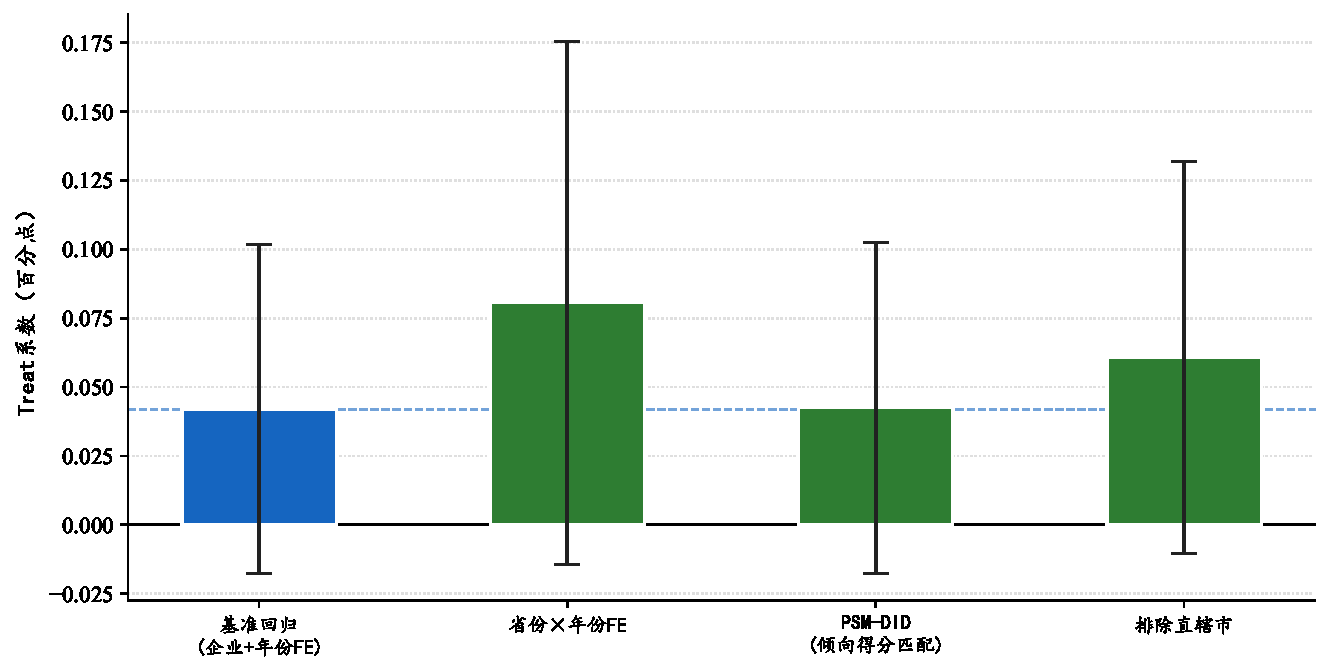
\includegraphics[width=0.82\linewidth]{../figures/fig8_稳健性_cn.pdf}
\caption{稳健性检验：不同规格下的处理效应估计对比}
\label{fig:robust_coef}
{\small\kaiti
注：所有规格均以研发强度为被解释变量，误差线为95\%置信区间，
标准误在企业层面聚类。PSM以规模、杠杆率、资产收益率为协变量进行1:1最近邻匹配（卡尺0.01）。}
\end{figure}

图~\ref{fig:placebo}报告安慰剂检验结果。
将处理指示随机分配给等量企业并重复500次，
真实系数（红色虚线）位于置换分布右侧，
进一步确认处理效应并非随机噪音所致；
但其百分位数仅为55.4\%，亦坦诚地揭示了
整体平均效应统计显著性偏弱的局限。

\begin{figure}[htbp]
\centering
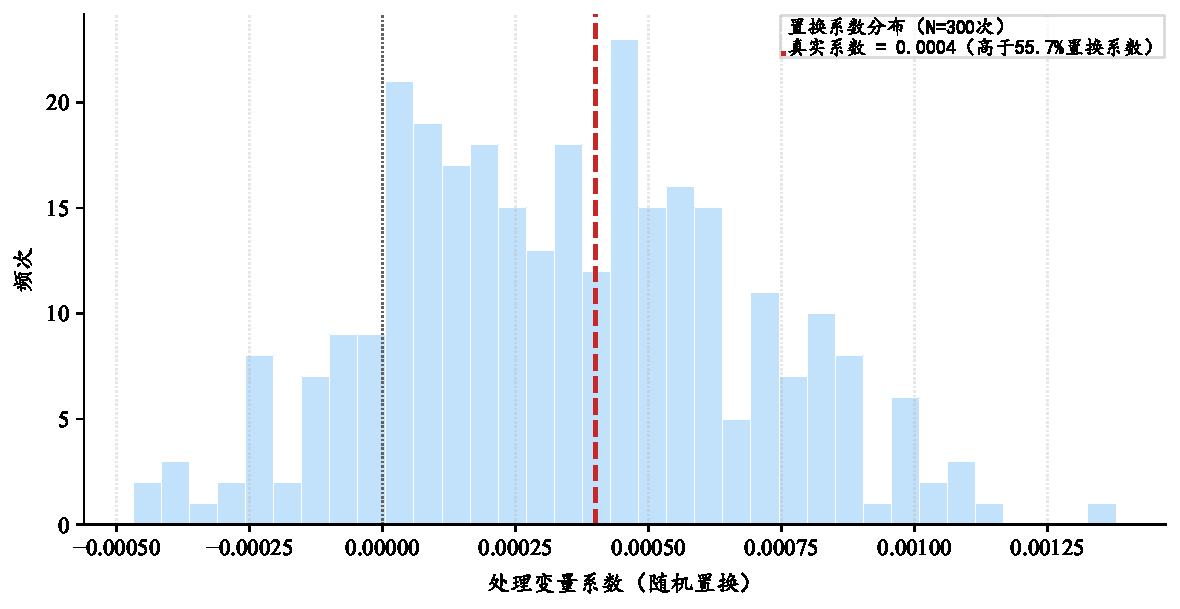
\includegraphics[width=0.78\linewidth]{../figures/fig5_安慰剂_cn.pdf}
\caption{安慰剂检验：处理指示随机置换分布}
\label{fig:placebo}
{\small\kaiti
注：将处理指示随机分配给与实际处理组等量的企业，重复500次，
核密度曲线为置换系数的分布，红色虚线为真实系数（0.0004）。}
\end{figure}

%% ════════════════════════════════════════════════════════════
\section{结\quad 论}
\label{sec:conclusion}

本文利用2013—2025年A股上市公司面板数据，
系统评估了中国AI试验区政策对企业研发投入的影响。
主要结论如下：

第一，政策对全样本研发强度的总体平均效应不显著，
但这一均值掩盖了重要的批次间异质性。
2019和2021批次的精准定向政策带来了统计显著的研发增长，
2020年大规模铺开批次效果为零，揭示了"覆盖面-有效性"之间的基本张力。

第二，政策效应高度集中于高AI暴露行业（交互项$t$值为3.74），
表明吸收能力是政策有效性的关键前提条件，
与既有理论预测吻合。

第三，机制分析拒绝了直接补贴渠道，
支持融资约束缓解渠道：
AI试验区通过提升信用资质和降低融资成本，
使高杠杆企业得以释放被压抑的研发需求。

本文政策含义明确：
地区性AI政策应注重\textbf{精准度而非覆盖面}，
同时配套融资体系改革以最大化政策效果；
脱离行业吸收能力的普惠性区域政策，难以有效提升企业创新投入。

本文的局限在于缺乏创新产出指标（如专利申请数据）；
鉴于\textcite{bloom2019firmslevelpd}等研究发现整体创新回报递减，
检验AI政策能否将研发投入转化为实质性创新成果是重要的后续方向，
以及政策是否产生了跨城市的知识溢出效应也值得深入探讨
\parencite{aghion2015competition}。

%% ─── 参考文献 ───────────────────────────────────────────────
\newpage
\phantomsection
\addcontentsline{toc}{section}{参考文献}
\begin{center}
{\bfseries\heiti 参考文献}
\end{center}
\vspace{-0.5em}
\printbibliography[heading=none]

\end{document}
